\begin{figure}[t]
    \centering
    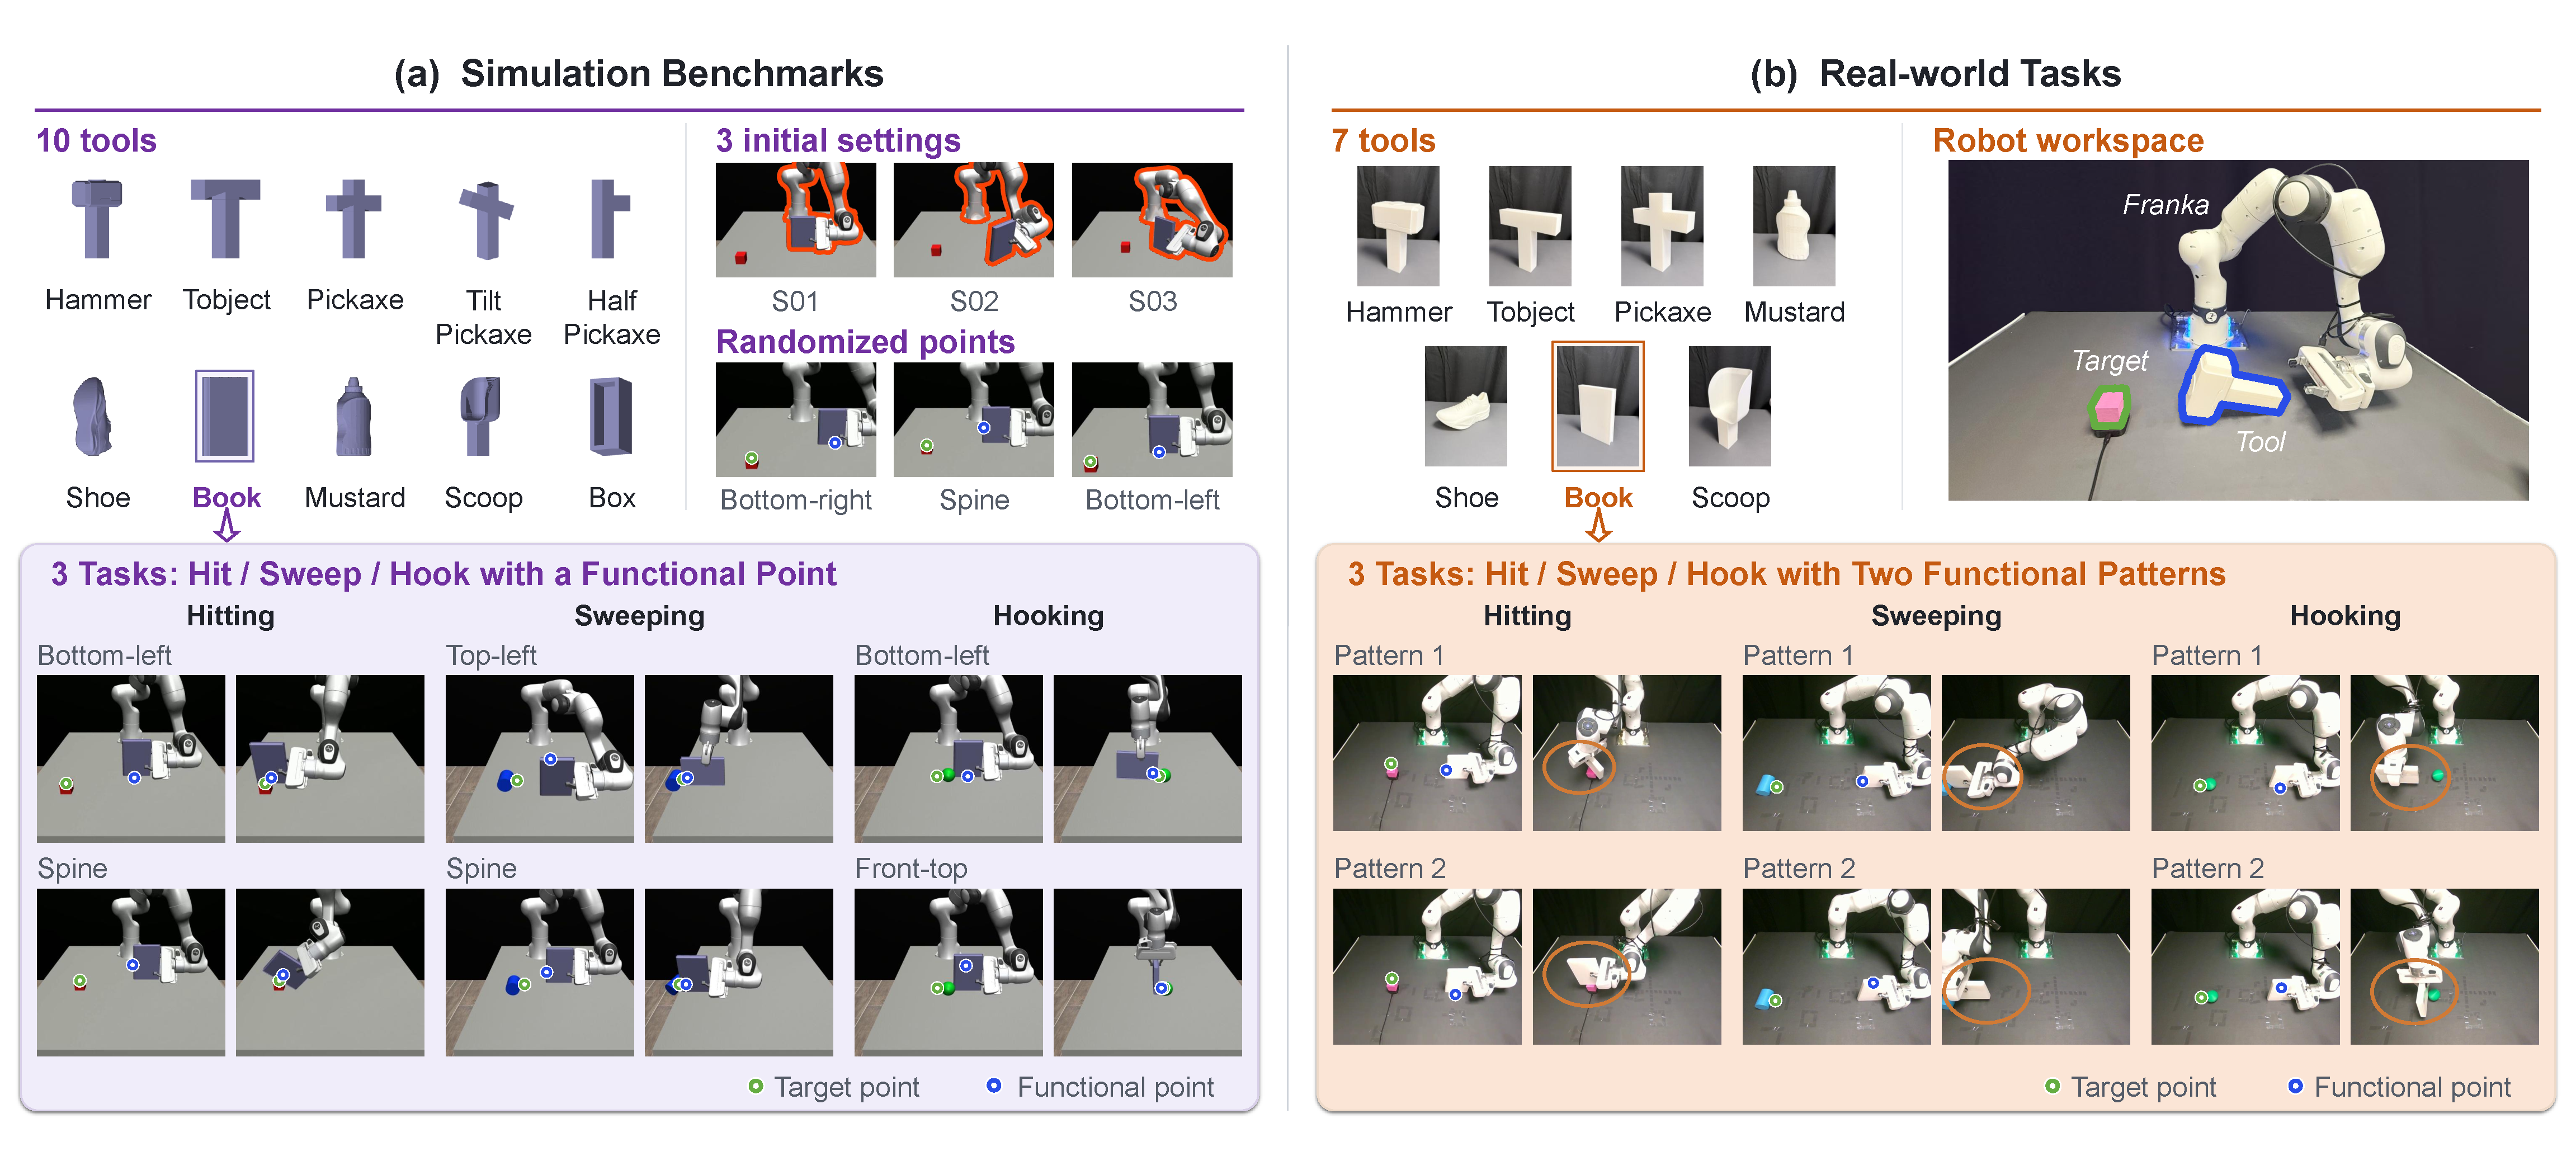
\includegraphics[width=0.95\linewidth]{figures/experiments_settings_v3.pdf}
    \caption{
   \textbf{Simulation Benchmark and Real-World Setting.} (a) The simulation benchmark contains 10 tools and three functions, including hitting, sweeping, and hooking, with multiple initial settings and randomized functional and target points. (b) The real-world benchmark uses a Franka robot with 7 tools and the same three functions, each evaluated under two functional patterns.}
    \label{fig:experiment_settings}
\end{figure}

\vspace{-15pt}
\section{{Experiments}}
\label{sec:experiments}

% highlight真机

Functional generalization remains largely underexplored in robotic manipulation.
In this work, we instantiate it across three representative tool-use functions, including hitting, sweeping, and hooking, and construct both simulation and real-world benchmarks to evaluate whether a policy can transfer each function to unseen tools with diverse geometries.
Specifically, we test four hypotheses underlying the central claims of this work:
% \begin{itemize}[leftmargin=*]
%     \item \textbf{H1}: Functional generalization requires an intermediate representation, not end-to-end mapping.
%     %Tested by the main comparison against FM and DP (Tab.~\ref{tab:simulation_results}).
%     \item \textbf{H2}: Among candidate intermediate representations, 2D keypoint trajectories best balance affordance expressiveness and action groundability.
%     % Tested by the representation ablation (Tab.~\ref{tab:ablation_intermediate_representation}).
%     \item \textbf{H3}: Keypoint trajectories must be function-aware; generic keypoint tracking is not enough.
%     % Tested by the comparison against ATM, which uses pretrained generic keypoints (Tab.~\ref{tab:simulation_results}).
%     \item \textbf{H4}: The two-stage design generalizes under moderate action-labeled tool diversity, making it a practical recipe for tool-use learning.
%     % Tested by the tool-diversity ablation (Tab.~\ref{tab:ablation_tool_generalization_setting}).
% \end{itemize}


\begin{itemize}[leftmargin=*]
    \item \textbf{H1}: Functional generalization benefits from an explicit, function-aware intermediate representation rather than direct perception-to-action mapping or generic motion cues.
    % \item \textbf{H1}: Functional generalization benefits from explicit function-aware motion guidance beyond direct perception-to-action mapping.
    \item \textbf{H2}: Among candidate intermediate representations, 2D keypoint trajectories best balance functional expressiveness and action groundability.
    
    \item \textbf{H3}: Functional generalization can be achieved with moderate action-labeled tool diversity.
    
    \item \textbf{H4}: Functional reasoning is scalable, which can benefit from more diverse action-free data and demonstrate greater autonomy through VLM-based functional point selection.
\end{itemize}


\subsection{Experimental setup}
\label{sec:experiments_setup}
% \textbf{Simulation Benchmark.}~~
% As shown in Fig.~\ref{fig:experiment_settings}, our simulation benchmark contains 7 tools, each with 3 different initial settings. 
% For each tool-setting pair, we collect 30 demonstrations using a four-stage Model Predictive Path Integral (MPPI) planner, resulting in 630 demonstrations in total. The MPPI planner generates an action trajectory by optimizing stage-dependent objectives that sequentially encourage the robot to lift the tool, move it toward the target, align the tool-specific hitting point with the target cube, and execute the final strike. In each demonstration, we randomly initialize the target cube position and sample the tool-specific hitting point along the tool boundary, requiring the policy to adapt its motion to both the tool geometry and the target location. In the main setting, all methods are trained on 4 tools, including hammer, tobject, pickaxe, and mustard, and evaluated on the remaining 3 unseen tools. During evaluation, each unseen tool is tested under three initial settings with 30 rollout episodes. A rollout is considered successful only if the robot strikes the target cube using the designated hitting point.

% \textbf{Simulation Benchmark.}~~As shown in Fig.~\ref{fig:experiment_settings}, our simulation benchmark contains 10 tools and three tool-use functions, including hitting, sweeping, and hooking, with three initial settings for each tool. 
% For each tool-setting-function combination, we collect 30 demonstrations using MPPI-based planners with function-specific objectives, resulting in 2,700 demonstrations in total. 
% In each demonstration, we randomize the target position and the tool-specific functional point, requiring the policy to adapt its motion to the tool geometry, functional point, and target configuration.
% In the main setting, all grounded execution policies are trained with action-labeled data
% from four seen tools, including hammer, tobject, pickaxe, and mustard, and evaluated on three unseen tools, including scoop, shoe, and book, across all three functions.
% During evaluation, each unseen tool is tested under three initial settings with 30 rollout episodes per setting.
% A rollout is considered successful only if the specified function is completed using the designated functional point: for \textit{hitting}, the selected hitting point must strike the red cube; for \textit{sweeping}, the selected sweeping point must push the blue cylinder; and for \textit{hooking}, the selected hooking point must hook the green ball inward. For the same tool and function, different functional points may be specified, e.g., using either the hammer head or handle for hitting.


\textbf{Simulation Benchmark.}~~
As shown in Fig.~\ref{fig:experiment_settings}, our simulation benchmark covers 10 tools and three functions, including hitting, sweeping, and hooking, with three initial settings per tool.
For each tool-setting-function combination, we collect 30 demonstrations using function-specific MPPI planners, totaling 2,700 demonstrations.
In the main setting, all methods are trained on action-labeled data from four tools (hammer, tobject, pickaxe, and mustard) and evaluated on three unseen tools held out from action-labeled training (scoop, shoe, and book) across all functions.
% In the main setting, all grounded execution policies are trained on action-labeled data from four seen tools (hammer, tobject, pickaxe, and mustard) and evaluated on three unseen tools (scoop, shoe, and book) across all functions.
Each unseen tool is evaluated under three initial settings with 30 rollouts per setting.
For each demonstration, we randomize the target position and designated functional point, with different points possible for the same tool and function (e.g., using the hammer head or handle for hitting).
A rollout is successful only if the specified function is completed using that point: \textit{hitting} requires the hitting point to strike the red cube, \textit{sweeping} requires the sweeping point to push the blue cylinder, and \textit{hooking} requires the hooking point to pull the green ball inward.




% \textbf{Real-World Setting.}~~
% We further construct a real-world benchmark on a Franka robot platform, as shown in Fig.~\ref{fig:experiment_settings}. 
% The real-world setting contains 3 tools: hammer, mustard, and book. 
% Each tool has two hitting patterns, and each pattern contains 20 expert demonstrations, resulting in 120 real-world trajectories.
% We train the policy on hammer and mustard and evaluate its functional generalization ability on the unseen book tool. 
% For each hitting pattern, we perform 20 real-world rollout trials. A trial is successful if the robot follows the specified hitting pattern and strikes the target.

% \textbf{Real-World Setting.}~~
% We further construct a real-world benchmark on a Franka robot platform, as shown in Fig.~\ref{fig:experiment_settings}.
% The benchmark covers 7 tools and the same three functions, with two functional patterns defined for each function.
% For each training tool and functional pattern, we collect 20 expert demonstrations.
% For hitting, we train the policies on hammer, pickaxe, and mustard and evaluate on three unseen tools: tobject, book, and shoe.
% For sweeping and hooking, we train the policies on hammer and mustard and evaluate on the unseen book.
% Each pattern is evaluated with 10 real-world rollout trials, and a trial is considered successful if the robot completes the specified function using the designated functional point.


\textbf{Real-World Setting.}~~
We further construct a real-world benchmark on a Franka robot platform.
The benchmark covers 7 tools and the same three functions, with two functional patterns defined for each function.
For each training tool and functional pattern, we collect 20 expert demonstrations.
For hitting, the policies are trained on hammer, pickaxe, and mustard and evaluated on three unseen tools (tobject, book, and shoe).
For sweeping and hooking, they are trained on hammer and mustard and evaluated on the unseen book.
Each functional pattern is evaluated with 10 real-world rollouts.
Unlike simulation, the designated functional point specifies the required functional pattern rather than serving as a point-level success criterion. A rollout is successful if the robot completes the specified function following the corresponding pattern.


% \textbf{Baselines.}~~We compare \algoname{} against three baselines covering end-to-end and keypoint-based policies. All baselines receive the same inputs as \algoname{}: visual observations, proprioceptive states, and the initial functional and target point positions. \textit{Flow-Matching (FM)}~\citep{lipmanflow} and \textit{Diffusion Policy (DP)}~\citep{chi2025diffusion} are end-to-end visuomotor policies that map observations directly to actions, serving as references for the perception-to-action gap (Sec.~\ref{sec:intro}). \textit{ATM}~\citep{wen2023any} also conditions on keypoint trajectories, but obtains them from a generic tracker pretrained on LIBERO-90 rather than a function-aware predictor, allowing us to test whether the gain comes from using keypoints or from predicting function-aware keypoint motion.

\textbf{Baselines.}~~
We compare \algoname{} against three baselines covering end-to-end and keypoint-based policies.
All baselines receive the same inputs as \algoname{}: visual observations, proprioceptive states, and the initial functional, target, and tool point positions.
\textit{Flow-Matching (FM)}~\citep{lipmanflow} and \textit{Diffusion Policy (DP)}~\citep{chi2025diffusion} are end-to-end visuomotor policies that map observations directly to actions, serving as references for the perception-to-action gap (Sec.~\ref{sec:intro}).
\textit{ATM}~\citep{wen2023any} conditions the execution policy on keypoint trajectories. Given the functional and target points, it uses its generic any-point trajectory model pretrained on LIBERO-90 to predict their trajectories. This serves as a keypoint-based baseline using generic trajectory modeling rather than explicitly predicting function-aware keypoint motion.


\textbf{Evaluation Metrics.}~~
All experiments report the success rate (SR) as the main evaluation metric, which is defined as the number of successful trials divided by the total number of rollout trials.


\begin{table}[ht]
\centering
\caption{\textbf{Simulation Results on Unseen Tools.} Success rate (SR) on three unseen tools across hitting, sweeping, and hooking. Each tool is evaluated under 3 settings with 30 rollouts per setting.}
\label{tab:simulation_results}
\small
\setlength{\tabcolsep}{3.0pt}

\resizebox{0.9\linewidth}{!}{
\begin{tabular}{lcccccccccccc}
\toprule
& \multicolumn{4}{c}{Hitting} 
& \multicolumn{4}{c}{Sweeping}
& \multicolumn{4}{c}{Hooking} \\
\cmidrule(lr){2-5}
\cmidrule(lr){6-9}
\cmidrule(lr){10-13}

Method 
& Scoop & Shoe & Book & Avg. 
& Scoop & Shoe & Book & Avg.
& Scoop & Shoe & Book & Avg. \\
\midrule

FM 
& 0.07 & 0.03 & 0.16 & \cellcolor{gray!15} 0.09 
& 0.49 & 0.23 & 0.19 & \cellcolor{gray!15} 0.30
& 0.22 & 0.06 & 0.14 & \cellcolor{gray!15} 0.14 \\

DP 
& 0.18 & 0.08 & 0.26 & \cellcolor{gray!15} 0.17 
& 0.49 & 0.18 & 0.13 & \cellcolor{gray!15} 0.27
& 0.12 & 0.06 & 0.08 & \cellcolor{gray!15} 0.09 \\

ATM 
& 0.12 & 0.06 & 0.06 & \cellcolor{gray!15} 0.08 
& 0.41 & 0.16 & 0.19 & \cellcolor{gray!15} 0.25
& 0.10 & 0.07 & 0.24 & \cellcolor{gray!15} 0.14 \\

\midrule

\algoname{} 
& \textbf{0.42} & \textbf{0.23} & \textbf{0.42} 
& \cellcolor{gray!15}\textbf{0.36} 
& \textbf{0.71} & \textbf{0.29} & \textbf{0.34} 
& \cellcolor{gray!15}\textbf{0.45}
& \textbf{0.29} & \textbf{0.17} & \textbf{0.24} 
& \cellcolor{gray!15}\textbf{0.23} \\

\bottomrule
\end{tabular}
}
\end{table}



\begin{table}[ht]
\centering
% \caption{\textbf{Real-world evaluation on unseen tools across different functions.}
% For hitting, the policy is trained on hammer, pickaxe, and mustard and evaluated on three unseen tools.
% For sweeping and hooking, the policy is evaluated on the unseen book under two configurations.}
\caption{\textbf{Real-World Results on Unseen Tools.} Success rate (SR) under two functional patterns for hitting, sweeping, and hooking. Hitting is evaluated on three unseen tools, while sweeping and hooking are evaluated on the unseen book, with 10 rollouts per pattern.}

\label{tab:real_world_results}
\small
\setlength{\tabcolsep}{2.0pt}

\resizebox{0.9\linewidth}{!}{
\begin{tabular}{lccccccccccccccc}
\toprule
& \multicolumn{9}{c}{\textbf{Hitting}}
& \multicolumn{3}{c}{\textbf{Sweeping}}
& \multicolumn{3}{c}{\textbf{Hooking}} \\
\cmidrule(lr){2-10}
\cmidrule(lr){11-13}
\cmidrule(lr){14-16}

& \multicolumn{3}{c}{Tobject}
& \multicolumn{3}{c}{Book}
& \multicolumn{3}{c}{Shoe}
& \multicolumn{3}{c}{Book}
& \multicolumn{3}{c}{Book} \\
\cmidrule(lr){2-4}
\cmidrule(lr){5-7}
\cmidrule(lr){8-10}
\cmidrule(lr){11-13}
\cmidrule(lr){14-16}

Method
& P01 & P02 & Avg.
& P01 & P02 & Avg.
& P01 & P02 & Avg.
& P01 & P02 & Avg.
& P01 & P02 & Avg. \\
\midrule

FM
& 0.00 & 0.60 & \cellcolor{gray!15} 0.30
& 0.50 & 0.00 & \cellcolor{gray!15} 0.25
& 0.00 & 0.20 & \cellcolor{gray!15} 0.10
& 0.30 & 0.00 & \cellcolor{gray!15} 0.15
& 0.20 & 0.00 & \cellcolor{gray!15} 0.10 \\

\algoname{}
& \textbf{0.60} & \textbf{0.80} & \cellcolor{gray!15}\textbf{0.70}
& \textbf{0.60} & \textbf{1.00} & \cellcolor{gray!15}\textbf{0.80}
& \textbf{0.20} & \textbf{0.60} & \cellcolor{gray!15}\textbf{0.40}
& \textbf{0.80} & \textbf{0.30} & \cellcolor{gray!15}\textbf{0.55}
& \textbf{0.90} & \textbf{0.30} & \cellcolor{gray!15}\textbf{0.60} \\

\bottomrule
\end{tabular}
}

\end{table}




\subsection{Main Results \& Analysis}

\textbf{Simulation Results.}~~
% As shown in Tab.~\ref{tab:simulation_results}, \algoname{} outperforms all baselines across hitting, sweeping, and hooking on unseen tools.
% Compared with the best baseline results of $0.17$, $0.30$, and $0.14$, it achieves average SRs of $0.36$, $0.45$, and $0.23$, respectively.
% The weak performance of FM and DP suggests that direct perception-to-action mapping struggles to adapt tool-specific motions to unseen geometries without tool-specific action supervision, while ATM shows that generic keypoint trajectories alone are insufficient to provide function-relevant motion guidance.
% Together, these results support \textbf{H1}: functional generalization benefits from an explicit, function-aware intermediate representation.
As shown in Tab.~\ref{tab:simulation_results}, \algoname{} outperforms all baselines across hitting, sweeping, and hooking on unseen tools.
Compared with the best baseline results of $0.17$, $0.30$, and $0.14$, it achieves average SRs of $0.36$, $0.45$, and $0.23$, respectively.
The weak performance of FM and DP suggests that direct perception-to-action mapping struggles to adapt tool-specific motions to unseen geometries without tool-specific action supervision.
Despite being conditioned on the designated functional and target points, ATM performs less effectively, suggesting that its generic keypoint predictor may fail to produce effective function-relevant motion guidance for diverse tool geometries.
Together, these results support \textbf{H1}: explicit function-aware intermediate representation provides useful guidance for functional generalization.


\textbf{Real-World Results.}~~
We test \algoname{} on the real-world benchmark across all three functions.
As shown in Tab.~\ref{tab:real_world_results}, \algoname{} consistently outperforms the FM baseline across all evaluated unseen-tool and functional-pattern settings. These results extend the evidence for \textbf{H1} to real-world manipulation, showing that function-aware keypoint plans provide more reliable guidance.
% For hitting, \algoname{} achieves average SRs of $0.70$, $0.80$, and $0.40$ on tobject, book, and shoe, compared with $0.30$, $0.25$, and $0.10$ for FM.
% On the unseen book, it further improves the average SR from $0.15$ to $0.55$ for sweeping and from $0.10$ to $0.60$ for hooking.
% These results extend the evidence for \textbf{H1} to real-world manipulation, showing that function-aware keypoint plans provide more reliable guidance.
%than direct perception-to-action mapping across diverse functions and unseen tools.

\textbf{Failure Case Analysis.}~~
We further examine representative baseline failures on the hitting function in both simulation and the real world.
As shown in Fig.~\ref{fig:qualitative-analysis}, the baselines exhibit three typical failure modes: \emph{pass over}, where the tool moves across the target without establishing the intended contact; \emph{imprecise hitting}, caused by insufficient fine-grained spatial alignment; and \emph{tool dropping}, associated with unstable or overly aggressive motions.
In the corresponding cases, \algoname{} successfully completes the task by predicting function-aware keypoint trajectories that guide the functional region toward the target with the appropriate motion and alignment.
Additional qualitative comparisons across hitting, sweeping, and hooking in both simulation and the real world are provided in App.~\ref{app:additional_experimental_results}.


\begin{figure}[ht]
    \centering
    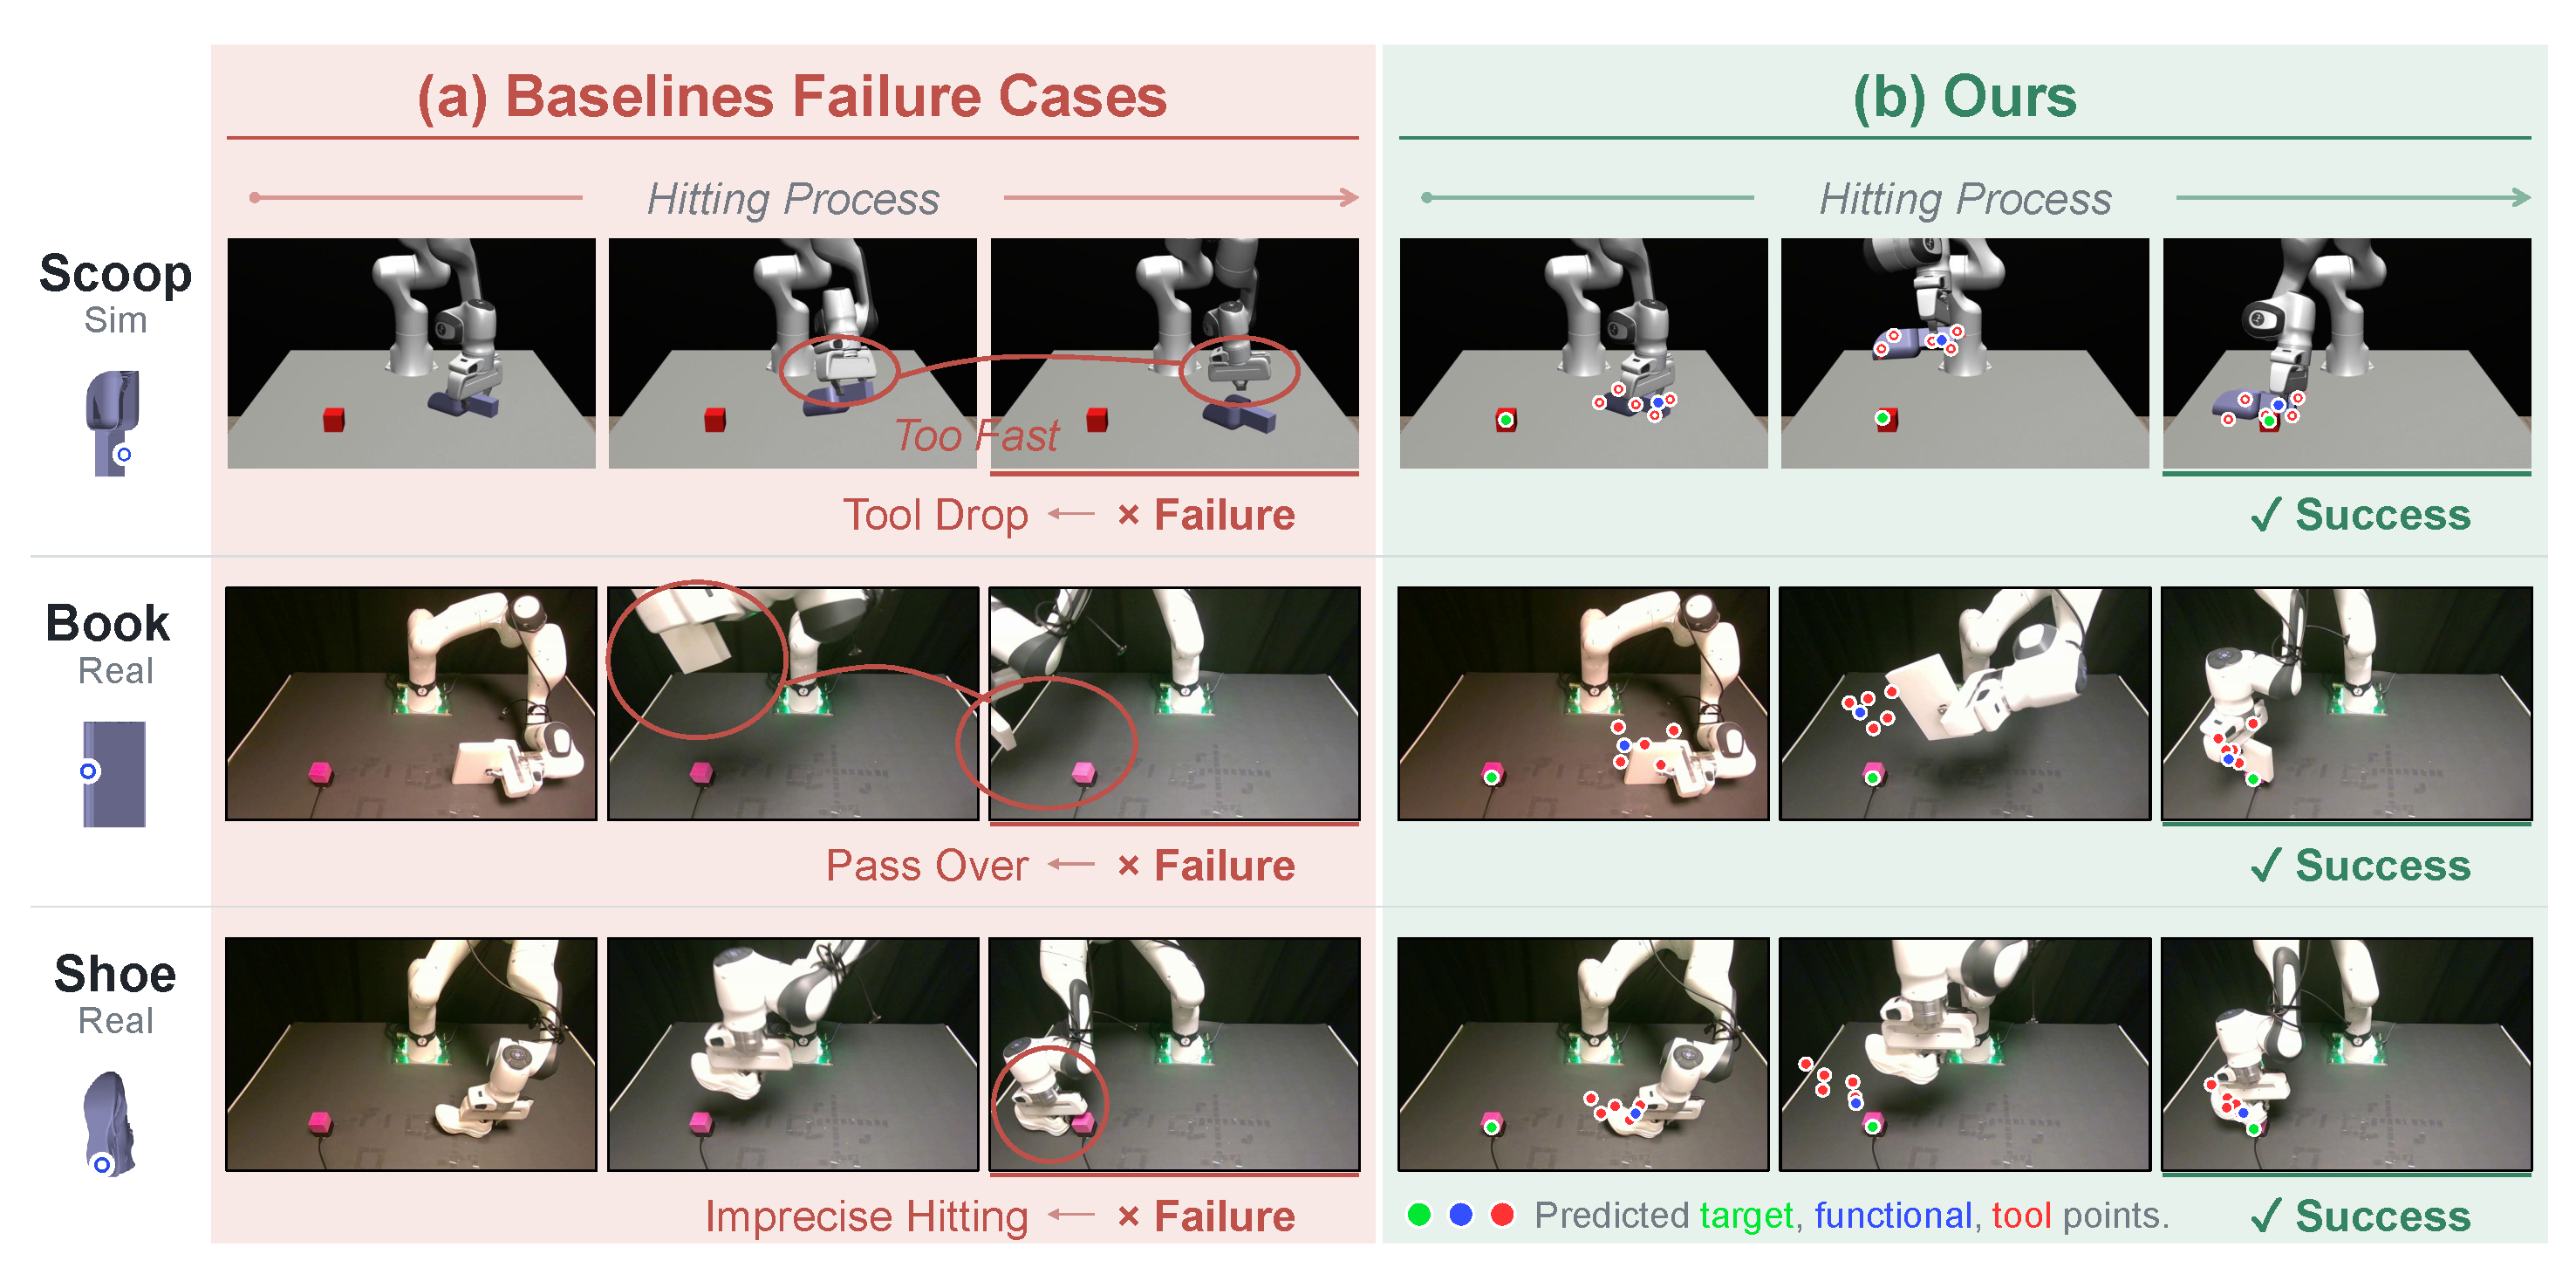
\includegraphics[width=0.82\linewidth]{figures/qualitative_results_v2.pdf}
    \caption{\textbf{Qualitative Comparison on Unseen Tools.} Representative baseline failure cases and successful rollouts of \algoname{} for hitting in simulation and the real world.}

    \label{fig:qualitative-analysis}
\end{figure}


\subsection{Ablation Studies}
% Beyond the main comparisons, we conduct two ablations to dissect the key design choices behind \algoname{}.
% Unless otherwise specified, all ablation experiments are conducted on the hitting function in simulation.
% First, we vary the functional intermediate representation while keeping the execution policy fixed, comparing affordance images, human video prompts, per-frame functional videos and object masks, and 2D keypoint trajectories to assess which representation best balances functional expressiveness and action groundability.
% The second ablation varies the diversity of action-labeled tools, training \algoname{} on 1, 4, or 7 tools and testing on the three unseen tools, to evaluate whether the two-stage design provides a practical recipe for functional generalization using moderate robotic data.
Beyond the main comparisons, we conduct two ablations on the key design choices of \algoname{}: the functional intermediate representation and the diversity of action-labeled tools.
Unless otherwise specified, all ablations are conducted on the hitting function in simulation.


\subsubsection{Effect of Functional Intermediate Representations.}

\begin{table}[ht]
\centering
\caption{\textbf{Ablation Results on Functional Intermediate Representations.} Success rate (SR) for hitting on unseen tools when different representations condition the same execution policy $\pi_{\mathrm{sys1}}$.}
\label{tab:ablation_intermediate_representation}
\small

\begin{tabular*}{0.9\linewidth}{
@{\extracolsep{\fill}}
llccc>{\columncolor{gray!12}}c
}
\toprule
Representation & Temporal input & Scoop & Shoe & Book & \cellcolor{white}Avg. \\
\midrule
None (FM) & -- & 0.07 & 0.03 & 0.16 & 0.09 \\
Affordance image & Static & 0.34 & 0.11 & 0.16 & 0.20 \\
Human video prompt & Pooled & 0.26 & 0.09 & 0.23 & 0.19 \\
\midrule
Per-frame video & Sequence & 0.28 & 0.13 & 0.29 & 0.23 \\
Per-frame object masks & Sequence & 0.37 & 0.16 & 0.43 & 0.32 \\
Keypoint trajectories & Sequence &
\textbf{0.50} & \textbf{0.31} & \textbf{0.67} & \textbf{0.49} \\
\bottomrule
\end{tabular*}

\end{table}

As discussed in Sec.~\ref{sec:Functional Intermediate Representations Selection}, we investigate the effect of functional intermediate representations by training and evaluating the execution policy $\pi_{\mathrm{sys1}}$ with pre-extracted representations as conditions.
Results in Tab.~\ref{tab:ablation_intermediate_representation} show that static affordance images and pooled human video prompts improve generalization, indicating that functional-region cues and motion demonstrations provide guidance.
Providing temporally varying representations improves performance, while object masks achieve stronger generalization by only retaining object-centric motion cues.
Among representations, 2D keypoint trajectories perform best, as they compactly encode fine-grained functional and target locations together with their structured motion over time.
These results support \textbf{H2}: keypoint trajectories best balance functional expressiveness and action groundability.



\subsubsection{Effect of Action-Labeled Tool Diversity.}
\begin{wraptable}{r}{0.54\linewidth}
\vspace{-0.8em}
\centering
\captionsetup{skip=4pt}
\caption{\textbf{Ablation on Action-Labeled Tool Diversity.} Success rate (SR) of \algoname{} when the execution policy $\pi_{\mathrm{sys1}}$ is trained with action-labeled data from $M=1 \text{,} 4 \text{,} 7$ tools and consistently evaluated on the same three unseen tools: scoop, shoe, and book.}
\label{tab:ablation_tool_generalization_setting}

\resizebox{0.95\linewidth}{!}{
\begin{tabular}{lcccc}
\toprule
\multirow{2}{*}{Method}
& \multicolumn{4}{c}{Tools} \\
\cmidrule(lr){2-5}
& Scoop & Shoe & Book & Avg. \\
\midrule
\algoname{} (1-to-3) & 0.14 & 0.10 & 0.23 & \cellcolor{gray!12} 0.16 \\
\algoname{} (4-to-3) & 0.42 & 0.23 & 0.42 & \cellcolor{gray!12} 0.36 \\
\algoname{} (7-to-3) & 0.39 & 0.27 & 0.52 & \cellcolor{gray!12} 0.39 \\
\bottomrule
\end{tabular}
}
\vspace{-0.8em}
\end{wraptable}
% Beyond the standard 4-to-3 setting, we vary the number of action-labeled training tools, while consistently evaluating on the same three unseen tools: scoop, shoe, and book.
% As shown in Tab.~\ref{tab:ablation_tool_generalization_setting}, increasing the training diversity from 1 to 4 tools substantially improves the average success rate from $0.16$ to $0.36$, while further increasing it to 7 tools yields only a marginal gain to $0.39$.
% This saturation is consistent with the role of System-1, which primarily grounds functional plans into executable actions rather than learning cross-tool functional reasoning. Therefore, moderate robotic data already provides sufficient coverage for action grounding, suggesting that further performance improvements increasingly depend on improving the System-2 functional planner.
% These results support \textbf{H3}: moderate action-labeled robotic data is sufficient to support functional generalization in our two-stage framework.
Beyond the standard 4-to-3 setting, we vary the number of action-labeled training tools while consistently evaluating on the same three unseen tools: scoop, shoe, and book.
As shown in Tab.~\ref{tab:ablation_tool_generalization_setting}, increasing the training diversity from 1 to 4 tools substantially improves the average SR from $0.16$ to $0.36$, while further increasing it to 7 tools yields a smaller gain to $0.39$.
These results support \textbf{H3}: functional generalization can be achieved with moderate action-labeled tool diversity in our two-stage framework.


% figure 5的文字放大一些。
\begin{figure}[ht]
    \centering
    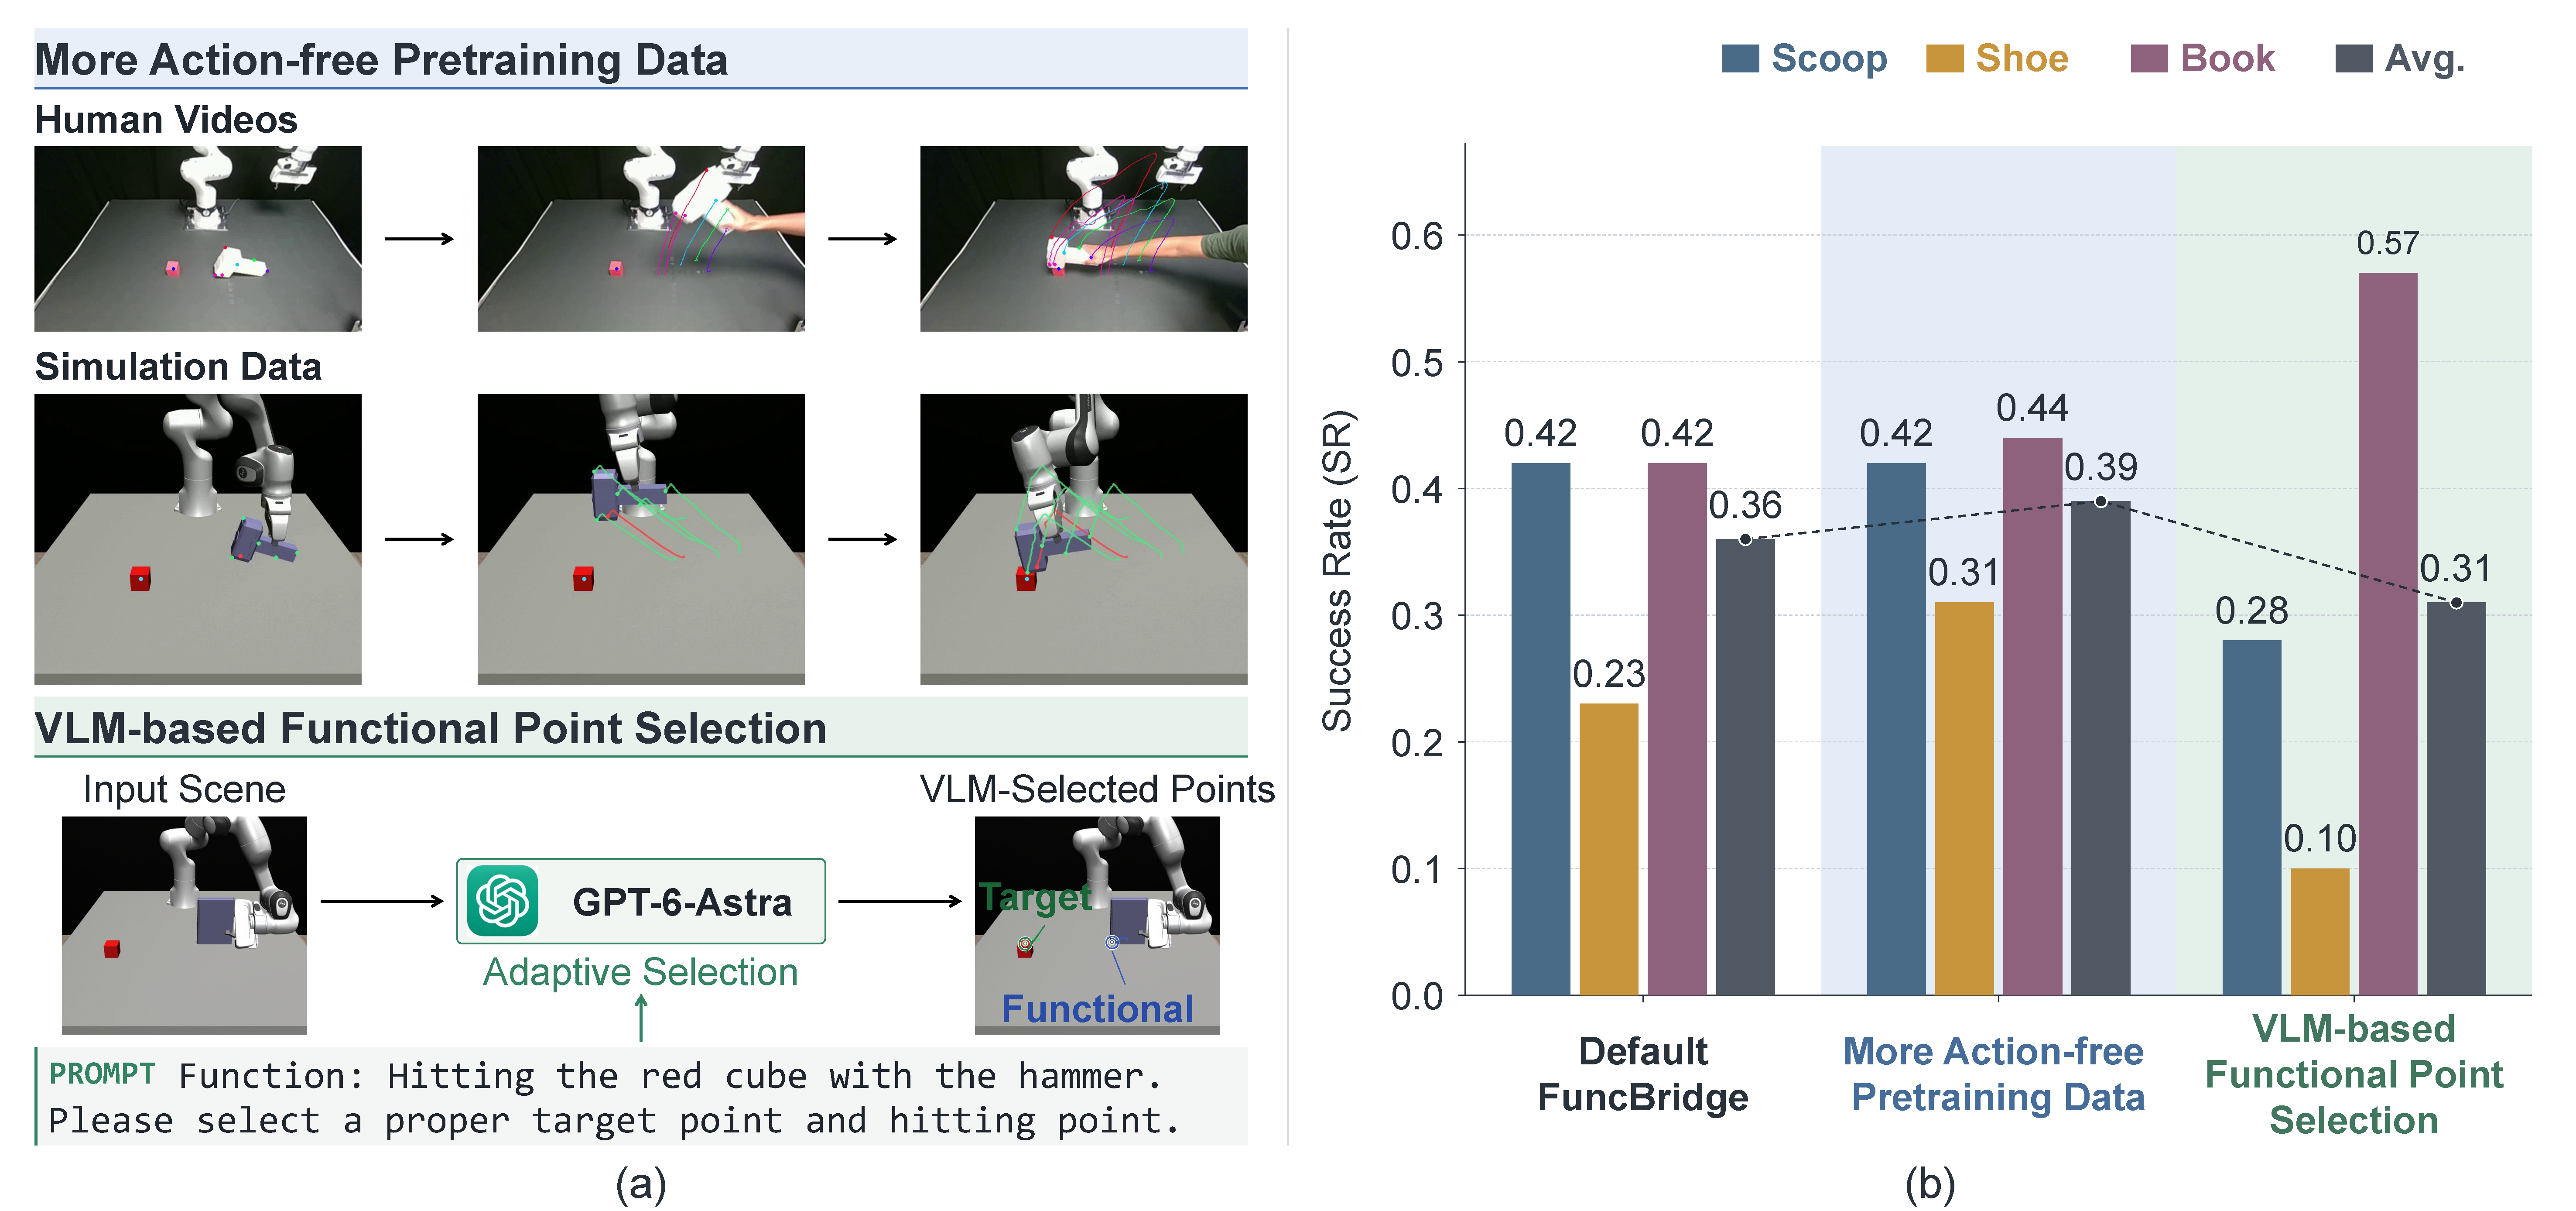
\includegraphics[width=0.95\linewidth]{figures/further_analysis_v2.pdf}
    \caption{\textbf{Scalability of \algoname{}.} (a) Extensions using human videos and VLM-based functional point selection. (b) Success rates on unseen tools for the default model and each extension.}

    \label{fig:further-analysis}
\end{figure}


% \subsection{Scalability of \algoname{}}
% \label{sec:scalability}

% Our default setting learns functional reasoning from action-free simulation videos and uses provided functional and target points at evaluation. We test \textbf{H4} through human-video pretraining and VLM-based point selection.

% \subsubsection{Scaling Action-Free Pretraining with Human Videos.}
% \label{sec:scalability-human-video}
% We augment the action-free pretraining data for $\pi_{\mathrm{sys2}}$ with 525 keypoint-annotated human hitting videos (App.~\ref{app:fir_extraction}), keeping the same four-tool action-labeled data for fine-tuning $\pi_{\mathrm{sys1}}$. Average SR increases from $0.36$ to $0.39$ (Fig.~\ref{fig:further-analysis}), showing that \algoname{} benefits from heterogeneous action-free data.

% \subsubsection{Flexible VLM-Based Functional Point Selection.}
% Given the observed scene and task instruction, GPT-6-Astra selects the tool's functional point and the target point for \algoname{}'s planning and execution. VLM-selected points achieve an average SR of $0.31$, versus $0.36$ with manually specified points (Fig.~\ref{fig:further-analysis}), supporting more autonomous tool use without manual point specification.

\subsection{Scalability of \algoname{}}
\label{sec:scalability}

Our default setting learns functional reasoning from action-free simulation videos, while the functional and target points are provided during evaluation.
We further examine \textbf{H4} by extending \algoname{} with multi-source action-free data and VLM-based function-relevant point selection.
% Our default setting learns functional reasoning from action-free tool-use videos collected within the simulation benchmark, while the functional and target points are provided during evaluation. We further examine whether \algoname{} can scale beyond these settings by leveraging multi-sourced action-free data and automatically identifying function-relevant points with a VLM agent. Together, these analyses support \textbf{H4}.
% Our default setting learns functional reasoning from action-free simulation videos, with functional and target points provided at evaluation.
% We further examine \textbf{H4} using multi-source action-free data and VLM-based point selection.

\subsubsection{Scaling Action-Free Pretraining with Human Videos.}
\label{sec:scalability-human-video}
As shown in Fig.~\ref{fig:further-analysis} (a), we additionally collect and annotate keypoints of 525 human videos for the hitting function (see App.~\ref{app:fir_extraction} for details).
Together with the original action-free data, these videos are used to pretrain $\pi_{\mathrm{sys2}}$, while $\pi_{\mathrm{sys1}}$ is fine-tuned with the same four-tool action-labeled robotic data.
As shown in Fig.~\ref{fig:further-analysis} (b), incorporating human videos improves the average SR from $0.36$ to $0.39$.
This result shows that \algoname{} can benefit from heterogeneous action-free data, suggesting the potential of broader data sources for functional reasoning.

\subsubsection{Flexible VLM-Based Functional Point Selection.}
% We further reduce the reliance on manually provided functional and target points by introducing a VLM agent.
% Given the observed scene and task instruction, GPT-6-Astra is prompted to adaptively select the functional point on the tool and the target point, which are then used by \algoname{} for functional planning and grounded execution.
% As shown in Fig.~\ref{fig:further-analysis}, VLM-selected points achieve an average SR of $0.31$, compared with $0.36$ using manually specified points.
% The relatively small performance gap suggests that the generalization capability of VLMs can be naturally combined with \algoname{} to enable more autonomous functional tool use without manually specifying function-relevant points.
% Given the observed scene and task instruction, GPT-6-Astra is prompted to adaptively select the functional point on the tool and the target point, which are then used by \algoname{} for functional planning and grounded execution.
% As shown in Fig.~\ref{fig:further-analysis}, VLM-selected points achieve an average SR of $0.31$, compared with $0.36$ using manually specified points.
% The relatively small performance gap suggests that the generalization capability of VLMs can be combined with \algoname{} to enable more autonomous functional tool use without manually specifying function-relevant points.
Given the observed scene and task instruction, GPT-6-Astra is prompted to adaptively select the functional point on the tool and the target point, which are then used by \algoname{} for functional planning and grounded execution.
A rollout is considered successful if the VLM-selected functional point is used to strike the target object, following the same hitting objective as the default setting.
As shown in Fig.~\ref{fig:further-analysis}, VLM-selected points achieve an average SR of $0.31$, compared with $0.36$ using manually specified points.
The performance gap mainly comes from VLM errors that select incorrect or unsuitable hitting points, such as the top side of a book.
Nevertheless, the results show that VLM-based point selection can be integrated with \algoname{} to reduce manual specification and support more autonomous functional tool use.
